\item \textbf{{[}HCI/PRELIM/9597/2016/P1/Q4{]} }

A program is to be written to represent and implement a linked list
of nodes. Each node contains a string data value and a pointer. The
pointers link the data items in alphabetical order. 

The unused nodes are linked as shown below. The first unused node
is the position where the next new data item is to be stored. 
\begin{center}
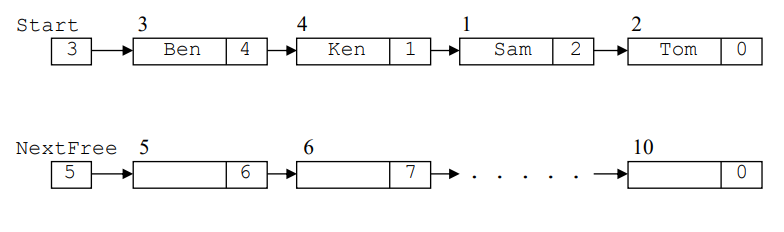
\includegraphics[width=0.65\paperwidth]{C:/Users/Admin/Desktop/Github/question_bank/LyX/static/img/9597-HCI-2016-P1-Q4-1}
\par\end{center}

The diagram shows the linked list with:
\begin{itemize}
\item the names \texttt{Sam}, \texttt{Tom}, \texttt{Ben} and \texttt{Ken}
(added in that order). 
\item the unused nodes linked together. 
\end{itemize}
The program will use a user-defined type \texttt{ListNode} for each
node defined as follows:
\noindent \begin{center}
\begin{tabular}{|c|c|c|}
\hline 
Identifier & Data Type & Description\tabularnewline
\hline 
\texttt{DataValue} & \texttt{STRING} & The node data\tabularnewline
\hline 
\texttt{PointerValue} & \texttt{INTEGER} & The node pointer \tabularnewline
\hline 
\end{tabular}
\par\end{center}

A linked list is implemented as an instance of the class \texttt{LinkedList}.
The class \texttt{LinkedList} has the following properties and methods:
\begin{center}
\begin{tabular}{|l|l|l|}
\hline 
\multicolumn{3}{|c|}{\texttt{Class: LinkedList}}\tabularnewline
\hline 
\multicolumn{3}{|c|}{Properties}\tabularnewline
\hline 
\texttt{\hspace{0.01\columnwidth}}Identifier & \texttt{\hspace{0.01\columnwidth}}Data Type & \texttt{\hspace{0.05\columnwidth}}Description\tabularnewline
\hline 
\texttt{Node} & \texttt{ARRAY{[}10{]} OF ListNode} & The linked list data structure -- data values and pointers. The array
index starts at 1. For testing purposes, the dataset has a maximum
of 10 items.\tabularnewline
\hline 
\texttt{Start} & \texttt{INTEGER} & Index position of the node at the start of the linked list. \tabularnewline
\hline 
\texttt{NextFree} & \texttt{INTEGER} & Index position of the next unused node.\tabularnewline
\hline 
\end{tabular}
\par\end{center}

\begin{center}
\begin{tabular}{|l|l|l|}
\hline 
\multicolumn{3}{|c|}{Methods}\tabularnewline
\hline 
\texttt{Initialise} & \texttt{PROCEDURE} & Sets all node data values to empty string. Set pointers to indicate
all nodes are unused and linked. Initialise values for \texttt{Start}
and \texttt{NextFree}.\tabularnewline
\hline 
\texttt{AddNode} & \texttt{PROCEDURE} & Add a new data item to the linked list. \tabularnewline
\hline 
\texttt{RemoveNode} & \texttt{PROCEDURE} & Remove a data item from the linked list.\tabularnewline
\hline 
\texttt{Display} & \texttt{PROCEDURE} & Display the current state of pointers and the array contents.\tabularnewline
\hline 
\texttt{IsEmpty} & \texttt{BOOLEAN FUNCTION} & Test for empty linked list. \tabularnewline
\hline 
\texttt{IsFull} & \texttt{BOOLEAN FUNCTION} & Test for no unused nodes.\tabularnewline
\hline 
\end{tabular}
\par\end{center}

\subsection*{Task 4.1 }

Write program code that repeatedly: 
\begin{itemize}
\item displays a menu with the following choices: 
\begin{enumerate}
\item[1.]  Add an item
\item[2.]  Remove an item 
\item[3.]  Output all pointers and data values 
\item[4.]  Exit 
\end{enumerate}
\item calls an appropriate procedure depending on the user\textquoteright s
choice. 
\end{itemize}

\subsection*{Evidence 15: }

Program code for Task 4.1. \hfill{}{[}5{]}

\subsection*{Task 4.2 }

Write program code for the classes \texttt{ListNode} and \texttt{LinkedList}.
Including the \texttt{Initialise}, \texttt{IsEmpty}, \texttt{IsFull}
and \texttt{Display} methods. The code should follow the specification
given. Do not attempt to write the methods \texttt{AddNode} and \texttt{RemoveNode}
at this stage.

\subsection*{Evidence 16: }

Program code for the \texttt{ListNode} and \texttt{LinkedList} classes
\hfill{}{[}10{]}

\subsection*{Task 4.3 }

Write code to create a \texttt{LinkedList} object in the main program. 

Run the program and select menu choice 3 to confirm the initial values
of the pointers and data values when the linked list is empty. 

\subsection*{Evidence 17:}

Screenshot confirming all values after initialisation of the \texttt{LinkedList}
object.\hfill{} {[}2{]}

Consider the \texttt{AddNode} method. The following pseudocode adds
a new data item to the linked list. The algorithm uses the variables
below:
\begin{center}
\begin{tabular}{|l|l|l|}
\hline 
\texttt{\hspace{0.01\columnwidth}}Identifier & \texttt{\hspace{0.01\columnwidth}}Data Type & \texttt{\hspace{0.05\columnwidth}}Description\tabularnewline
\hline 
NewItem & STRING & New data item input by the user\tabularnewline
\hline 
Found & BOOLEAN & lags to TRUE when the position at which to insert the new item has
been found\tabularnewline
\hline 
Current & INTEGER & array index position during list traversal\tabularnewline
\hline 
Previous & INTEGER & Previous array index position during list traversal\tabularnewline
\hline 
Temp & INTEGER & Temporary storage of pointer value\tabularnewline
\hline 
\end{tabular}
\par\end{center}

\noindent %
\noindent\begin{minipage}[t]{1\columnwidth}%
\texttt{PROCEDURE AddNode}

\texttt{\qquad{}INPUT NewItem}

\texttt{\qquad{}Node{[}NextFree{]}.DataValue = NewItem}

\texttt{\bigskip{}
}

\texttt{\qquad{}Temp = NextFree }

\texttt{\qquad{}NextFree = Node{[}NextFree{]}.PointerValue }

\texttt{\bigskip{}
}

\texttt{\qquad{}\# traverse the list to find the position to }

\texttt{\qquad{}\# insert the new item }

\texttt{\qquad{}Found = False }

\texttt{\qquad{}Current = Start }

\texttt{\qquad{}Previous = 0}

\texttt{\bigskip{}
}

\texttt{\qquad{}WHILE NOT Found AND Current != 0 }

\texttt{\qquad{}\qquad{}IF NewItem > Node{[}Current{]}.DataValue}

\texttt{\qquad{}\qquad{}\qquad{}THEN}

\texttt{\qquad{}\qquad{}\qquad{}\qquad{}\# move on to the next
node }

\texttt{\qquad{}\qquad{}\qquad{}\qquad{}Previous = Current }

\texttt{\qquad{}\qquad{}\qquad{}\qquad{}Current = Node{[}Current{]}.PointerValue}

\texttt{\qquad{}\qquad{}\qquad{}ELSE }

\texttt{\qquad{}\qquad{}\qquad{}\qquad{}Found = True }

\texttt{\qquad{}\qquad{}ENDIF}

\texttt{\qquad{}ENDWHILE}

\texttt{\bigskip{}
}

\texttt{\qquad{}IF Previous = 0 }

\texttt{\qquad{}\qquad{}THEN }

\texttt{\qquad{}\qquad{}\qquad{}\# new item will become the start
of the list}

\texttt{\qquad{}\qquad{}\qquad{}Start = Temp }

\texttt{\qquad{}\qquad{}\qquad{}Node{[}Temp{]}.PointerValue = Current }

\texttt{\qquad{}\qquad{}ELSE}

\texttt{\qquad{}\qquad{}\qquad{}\# new item is between previous
and current }

\texttt{\qquad{}\qquad{}Node{[}Previous{]}.PointerValue = Temp}

\texttt{\qquad{}\qquad{}Node{[}Temp{]}.PointerValue = Current }

\texttt{\qquad{}ENDIF }

\texttt{ENDPROCEDURE}%
\end{minipage}

Identifier Data Type Description F Current Note: The above pseudocode
is available in the text file \texttt{PSEUDOCODE\_TASK\_4\_4.txt}

\subsection*{Task 4.4 }

Write code to implement the \texttt{AddNode} method for the \texttt{LinkedList}
class. 

You may use the text file \texttt{PSEUDOCODE\_TASK\_4\_4.txt} as a
basis for the writing of your code.

The main program should check each time that the \texttt{LinkedList}
object is not full before using the \texttt{AddNode} method.

Run the program as follows: 
\begin{itemize}
\item Menu choice 1 four times, inputting the data values:

\texttt{Sam}, \texttt{Tom}, \texttt{Ben}, \texttt{Ken} in that order. 
\item Menu choice 3 to display.
\end{itemize}

\subsection*{Evidence 18: }

Your program code for Task 4.4. \hfill{}{[}5{]}

\subsection*{Evidence 19: }

Screenshot showing the pointers and the addition of the four nodes
to the linked list. \hfill{}{[}2{]}

\subsection*{Task 4.5 }

Write code to implement the \texttt{RemoveNode} method for the \texttt{LinkedList}
class. 

The main program should check each time that the LinkedList object
is not empty before using the \texttt{RemoveNode} method. Node removed
from the linked list should be returned to the NextFree list. 

Run the program as follows: 
\begin{itemize}
\item Menu choice 1 four times, inputting the data values: 

\texttt{Sam}, \texttt{Tom}, \texttt{Ben}, \texttt{Ken} in that order. 
\item Menu choice 2 two times, inputting the data values: 

\texttt{Sam}, \texttt{Ben} in that order.
\item Menu choice 3 to display. 
\end{itemize}

\subsection*{Evidence 20: }

Your program code for Task 4.5. \hfill{}{[}6{]}

\subsection*{Evidence 21: }

Screenshot showing the pointers and data values after the addition
of the four nodes followed by the removal of two nodes to the linked
list. \hfill{}{[}2{]}